
 \subsection{Discrete Particle Model}
 Discrete Particle Model simulates particle motion by applying forces and torques which derives from particle-particle interactions and external influences, on the basis of the given contact law. It performs calculations of kinematics that a given particle $i$ exerts on other particle $j$, for each particle in the system, among with the peripheral factors such as gravity and walls. To achieve this results, the particles are assumes to be (1) undeformable - deform therefore implemented as overlap, (2) unbreakable, (3) all internal interactions are due to particle-particle interaction, (4) Each particle pair $i, j$ has only one contact point $c_{ij}$ which the forces and torques act on, and (5) all external forces and torques are either body forces and torques or by interacting with a wall~\cite{MercuryDPM}. 

\subsubsection{Contact Laws}
For each particle $i$ on the system, Eq. \ref{eq:force} describes the internal and external forces, and Eq.~\ref{eq:torque} describes the torque acting on it \cite{MercuryDPM}:

\begin{equation} \label{eq:force}
 F_i = \sum_{j=1}^{n_p} F_{ij} + \sum_{k=1}^{n_w} F_{ik}^w + F_i^b
\end{equation}

\begin{equation} \label{eq:torque}
 \tau_i = \sum_{j=1}^{n_p} r_{ij}F_{ij} + \tau_{ij} + \sum_{k=1}^{n_w} r_{ik}F_{ik}^w + \tau_{ik}^w +\tau_{i}^{b} 
\end{equation}

With $F_{ij}$ interparticle forces, $F_{ik}^w$ the interaction force between each wall and the particle, $n_p =$ number of particles, $n_w =$ number of walls, $F_i^b$ body forces i.e., gravity, and $r_{ij}$ as the branch vector, which connects the particle position $r_i$ with the contact point $c_{ij}$ . The same hold for torques equation, with $\tau$ as torque. 

The contact law used in the simulations is the Linear Spring-Dashpot model, implemented in MercuryDPM as 
\texttt{LinearViscoelasticFrictionReversibleAdhesiveSpecies}. It defines the interaction between two particles $i$ and $j$ as a damped harmonic oscillator \cite{LSD-info}:

\begin{equation}
 F_{ij}^n=\begin{cases}
 k_n \delta_{ij}^n + \gamma_n v_{ij}^n &\text{if } \, \delta_{ij}^n > 0, \\
 0 \quad &\text{else, } \, \\
 \end{cases}
\end{equation}

In this equation, $k_n > 0$ represents spring stiffness, $\gamma_n \geq 0$ represents the damping coefficient, $v_n$ the normal vector, and $\delta_{ij}^n$ is the overlap between the particles. Two particles interact with each other if and only if they overlap. This contact model is simple, has an analytic solution, and is less computationally expensive \cite{NAVARRO2013}, while also suitable for large particles \cite{MercuryDPM}. In addition to particle-particle interactions, the current contact law also considers sliding friction, rolling friction, and adhesion. While sliding friction is defined as the force that acts in the tangential direction between two particles when they collide and resist lateral motion, rolling friction resists the angular motion of the particles (see equation~\ref{eq:sliding},~\ref{eq:rolling}).


\noindent
\begin{tabularx}{\linewidth}{@{}XX@{}}
 \begin{equation} \label{eq:sliding}
 |F_{ij}^t| \leq \mu^lF_{ij}^n
 \end{equation}
 &
 \begin{equation}\label{eq:rolling}
 \tau_{ij}^{\text{ro}} \leq \mu^{\text{ro}} \alpha^{\text{eff}}_{ij} F_{ij}^n
 \end{equation}
\end{tabularx}

With $F_{ij}^t$ and $\tau_{ij}^{\text{ro}}$ as the forces in the tangential direction, and rolling torques, respectively. When the lateral forces reach a particular threshold, the particle will begin to slide. The sliding motion is modeled using the Coulomb yield criterion, which cuts off the elastic displacement when it reaches a specific fraction (sliding friction $\mu^l$) of the normal force. The same applies to the rolling torque: it is cut off when it reaches a certain level, defined by the rolling friction $\mu^{\text{ro}}$. Finally, the adhesive forces model is defined as: 

\begin{equation}
 F_{ij}^a=\begin{cases}
 -F^a_{\text{max}} &\text{if } \, \delta_{ij}^n > 0, \\
 -F^a_{\text{max}} - k_c \delta_{ij}^n &\text{if } \, -F^a_{\text{max}} / k_c \leq \delta_{ij}^n < 0, \\
 0 \quad &\text{else, } \, \\
 \end{cases}
\end{equation}

The adhesive forces are reversible, i.e., equal during loading and unloading. The maximum adhesion force $-F^a_{\text{max}}$ is calculated using the bond number:

\begin{equation}\label{eq:bond}
    F^a_{\text{max}} = gm_{\text{50}}\text{Bo} 
\end{equation}

With $g$ denotes the gravitational acceleration, and $m_{50}$ is the average mass of the particles. More details about the sliding, rolling friction, and adhesion can be found in~\cite{MercuryDPM} and~\cite{LSD-info}. 
\subsubsection{Angle of Repose measurement}

In MercuryDPM, Static AoR is measured by a hollow cylinder simulation, consisting of two cylinders (instead of one cylinder and one plate in Fig.~\ref{fig:StaticAoR}), with the cylinder's diameter. For simplicity, all particles in the simulation are assumed to be a perfect sphere. After all the particles are poured into the cylinder, it is let to rest until the bulk's kinetic energy is less than $1\%$ compared to the potential energy (steady-state condition). At this point, the top cylinder is removed, and all the particles that have fallen out of the bottom cylinder below $z = 0$ are deleted. This will result in a cone-shaped heap of particles and a drastic increase in kinetic energy due to gravity. The heap will be rested again until it reaches a steady-state condition, as mentioned above, and then Static AoR can be measured. The measurement will be done twice since the system's kinetic energy can be increased again after the first measurement. Figure~\ref{fig:MercuryAoR} demonstrates an example simulation of MercuryDPM. 


\begin{figure}[H]
    \centering
    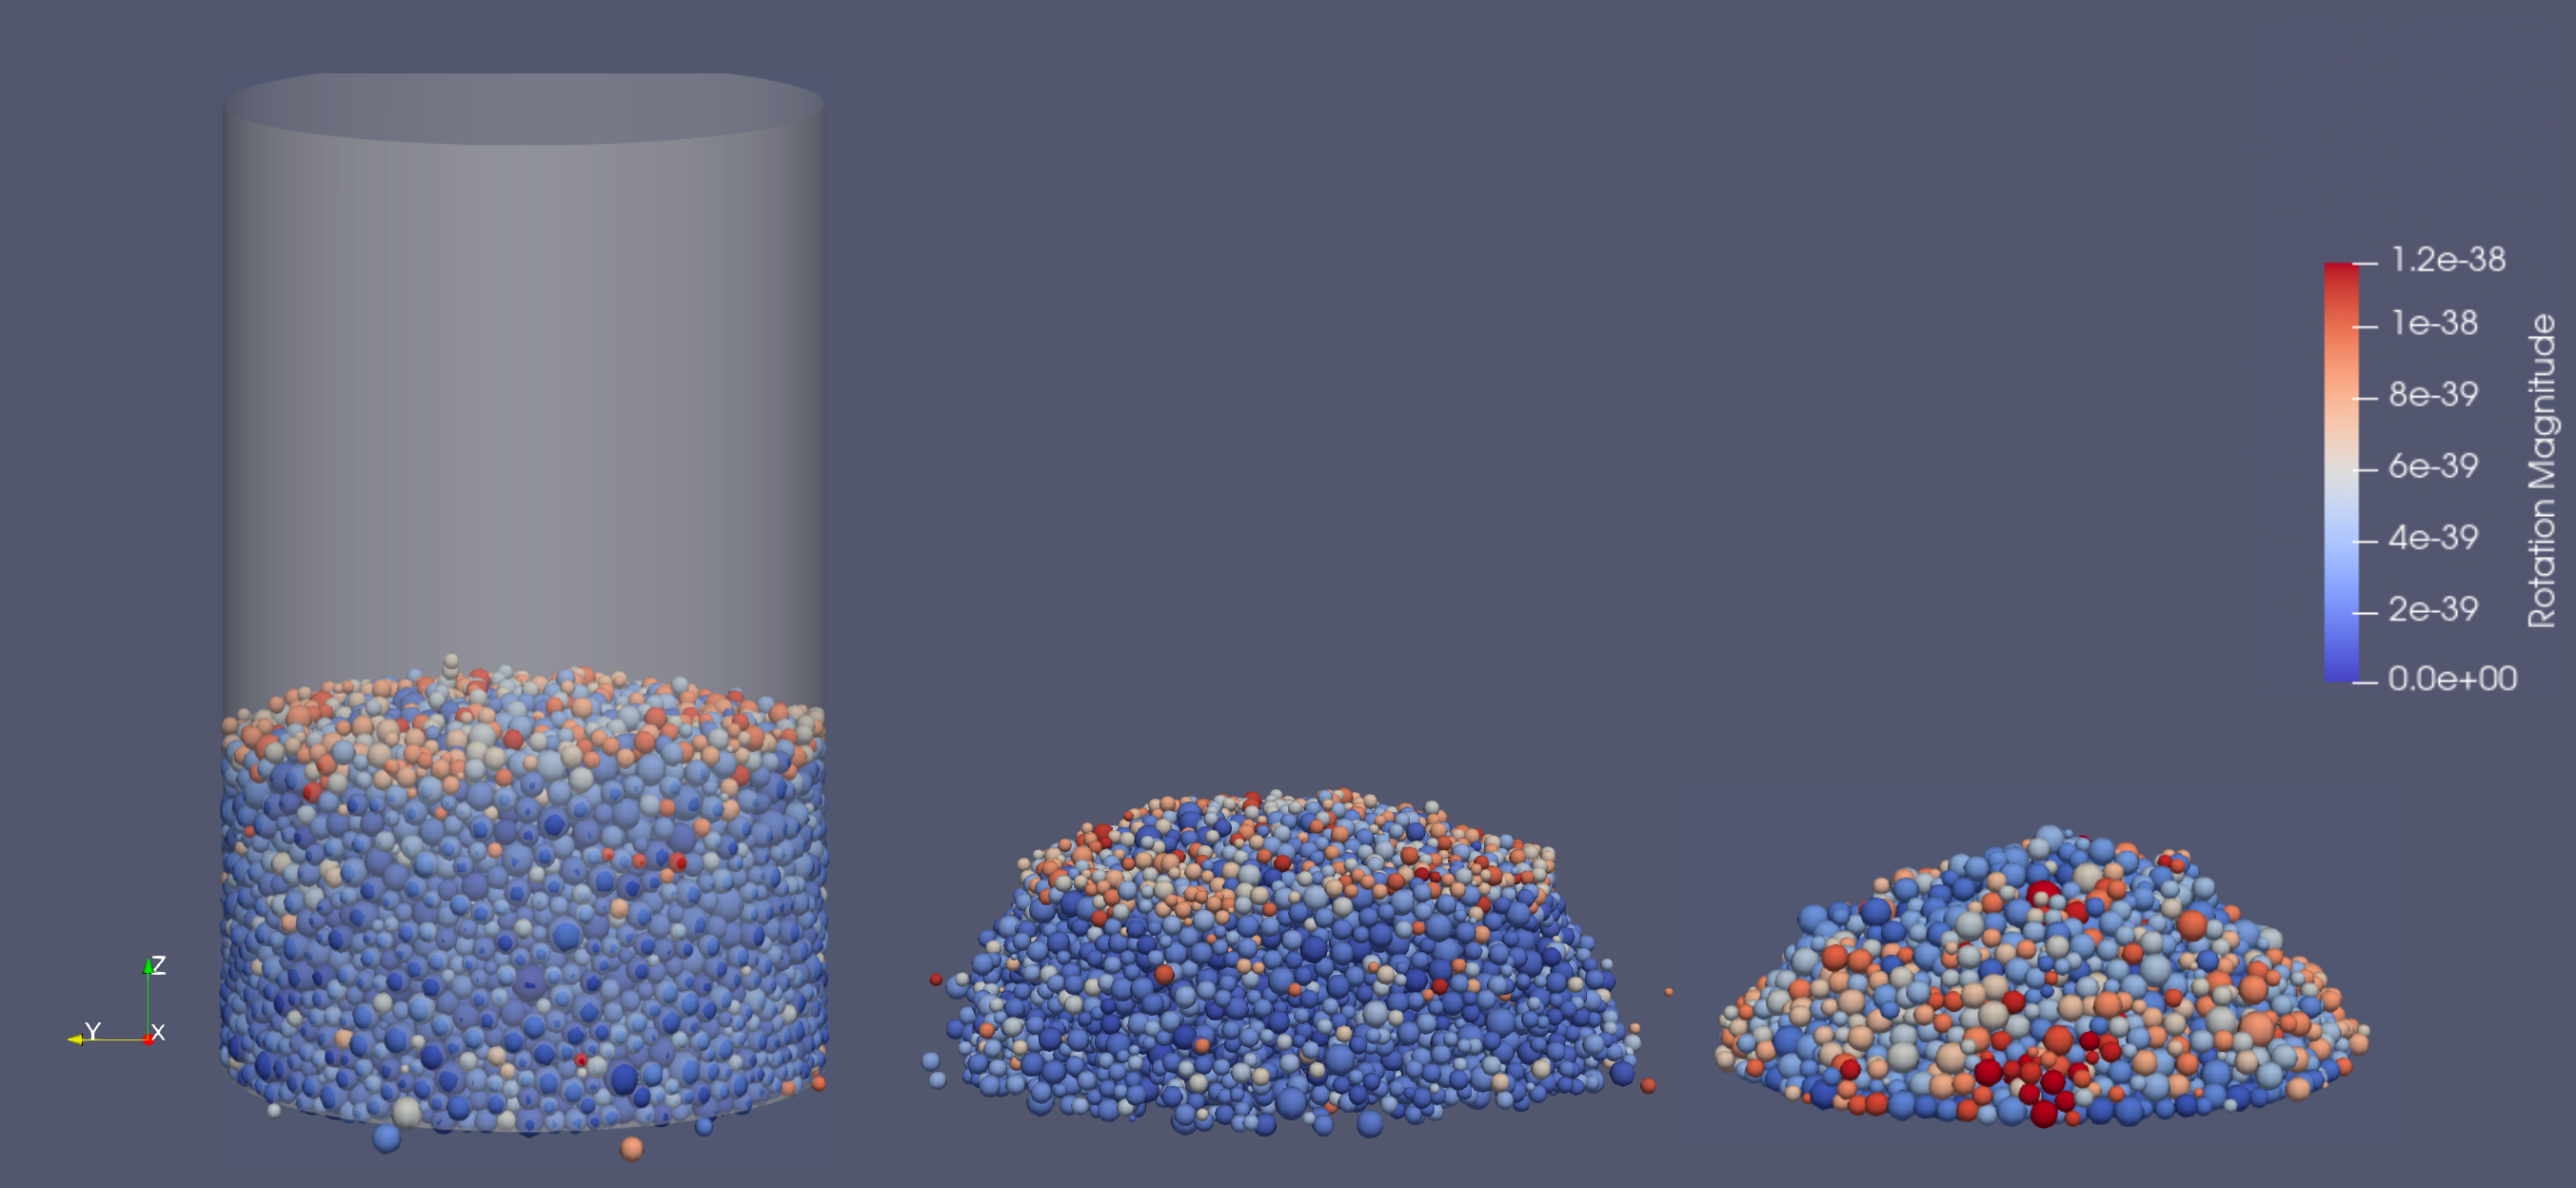
\includegraphics[scale=0.16]{AoRSim.png}
    \caption{Angle of Repose simulation on MercuryDPM. From left to right: Initial fill stage, wall removed, and final stage.}\label{fig:MercuryAoR}
\end{figure}
